% !TeX spellcheck = en_US
\section{AutoCompose}
\label{sec:630_autocompose}
AutoCompose takes the decisions generated by CrowdCompose and learns the composition patterns. 
Composition decisions are split into two separate steps, according to the pattern described in Section~\ref{sec:615_concept}: first, into the selection of the next video view, and then the time when it should be integrated into the composed video.
For automatic prediction, the machine learning algorithm \ac{SVM-HMM}, a support vector machine combined with a hidden Markov model, is chosen.
\subsection{SVM-HMM}
As an efficient sequence tagging learning algorithm, an \ac{SVM-HMM} is selected to understand the temporal sequence of shots in a composed video.
The concept of \ac{SVM-HMM} relies on the work of Altun et al. who show that it can outperform \ac{HMM} for sequence prediction in both learning time and accuracy~\cite{Altun2003}.
In recent years, further proposals have been made to increase the speed~\cite{Tsochantaridis2004,Tsochantaridis2005} and improve \ac{SVM} internals such as a novel cutting plane approach for the \ac{SVM-HMM}~\cite{Joachims2009}.

Sequence tagging as video composition requires an analysis of the historic decisions to predict the next, best view and a suitable shot duration.
The focus of AutoCompose lies on the video track, as it is assumed that the audio track shall only be switched if the audio quality suffers from major degradations~\cite{Wu2015}.
This is ensured using the filter stage.

An \ac{SVM-HMM} trains a model for an input sequence of feature vectors $x=(x_1,x_2,...,x_n)$ which can predict the sequence of tags $y=(y_1,y_2,...,y_n)$.
The \ac{SVM} is used for the formulation of the \ac{HMM}. 
The trained model of an \ac{SVM-HMM} is isomorphic to a k-th order \ac{HMM}. 
A major advantage of an \ac{SVM-HMM} in comparison to the classical \ac{HMM} is that the observation variables $x_1,x_2,...,x_n$ can be feature vectors and not only atomic values. 
This is leveraged as the input vector for the proposed composition algorithm consists of multiple input features.

A trained model predicts the next tag sequence $y$ as:
\begin{equation}
y = argmax_y {\sum_{i=1}^{n}[\sum_{j=1}^{k} (x_i \times w_{y_{i-j}...y_i}) + \phi t(y_{i-j},...,y_i) \times w_t]}
\end{equation}
 Here, $w_{y_{i-j}...y_i}$ represents the emission vector, which is known from \ac{HMM} and learned for each tag sequence $y_{i-j}...y_i$. 
 The transition vector, also known from \ac{HMM}, is represented by $w_t$ and gives the weights for the transitions between different tags.
 $\phi t(y_{i-j},...,y_i)$ represents a single value vector set to 1 to solve the sequence $y_{i-j}...y_i$.
\subsection{Features for AutoCompose}
Different features are used in an \ac{SVM-HMM} to describe the video views.
These characteristics are chosen as they influence how a video is composed. 
In detail, they influence the selection of the next view and its duration in the composed video.
In an initial step, the view selection fuses the location of the current view, the genre of the video composition, and content characteristics.
The video quality and the recording location determine the shot duration in the second step. 
\subsubsection{Location in the Scene Model}
Inputs for the \ac{SVM-HMM} (see Figure~\ref{fig:630_viewSelection}) are the location and the orientation of a recorder classified in the scene model, as proposed in Figure~\ref{fig:617_ac_location} and Section~\ref{sec:617_recordingQualityLocation}.
This represents a $3\times3$ field, including outlier regions with 11 states for the location.
The value of the distance and angle are combined into atomic string values, e.g., a recording at the front right side as "fr".
\subsubsection{Genre}
From professional compositions, it is known that the genre of a video has a major effect on the composition that is conducted. 
This affects the length a video view, as well as which video view shall be selected next.
A limited set of genres are selected that are common in today's \ac{UGV}: Sports (s), Music (m), Performing Arts (pa), Speech/Lecture/News (le), and other (o).
The genres are represented as a single atomic genre string. 
The set of genres can be extended but that would require a retraining of the models.
Each composition can be initially classified into a genre, e.g., by workers in CrowdCompose or by automatic genre classification algorithms~\cite{Cricri2014}.
During a composition, the genre type may change, e.g., from music to speech.

\subsubsection{Visual Features}
To train the composition model, the composed video as well as all available views from CrowdCompose, are analyzed using computer vision algorithms.
These algorithms extract features and combine them with the data from the filter stage to learn composition patterns.
Thus, the features assume that the content of the recorded scene and each view significantly affects the composition decision. 
The filter stage has ensured that a suitable quality is available in each view, and cinematographic rules are followed.

Visual features are chosen that describe video views for a certain duration.
The \ac{ITU}-T P.910~\cite{ITU-J2008} and Hasler et al.~\cite{Hasler2003} have shown for video quality assessment that a classification of different video sequences is possible by describing the structure, motion, and colors.
This motivates the selection of the \ac{SI} for the description of structural information, \ac{TI} for describing the motion, and the \ac{Co} for the number of colors.
\ac{SI} and \ac{TI}, as proposed by \ac{ITU}-T P.910~\cite{ITU-J2008}, and the colorfulness of selected video frames~\cite{Hasler2003} represent the content of a video by classifying each video view according to the amount of structures (edges), the motion and the different colors it captures.

\ac{SI} applies a Sobel filter on each video frame $F_n$ from which the standard deviation of the pixel values is calculated when inspecting its luminance plane.
\begin{equation}
\begin{split}
SI = max_{t}\{{\sigma_{space}[Sobel(F_{n})]}\}
\end{split}
\end{equation}

\ac{TI} is calculated in a similar manner by considering the motion between to Sobel-filtered frames as  $M_n(i,j) = F_n (i,j) - F_{n-1}(i,j)$.  
The indices $i$ and $j$ represent the row and the column of the frame pixel inspected. 
\begin{equation}
TI = max_{t}\{{\sigma_{space}[M_n(i, j)]}\}\end{equation} 

As a third criterion, the \ac{Co} shows the perceptual differences in terms of colors in video sequences. 
It was proposed by Hasler et al.~\cite{Hasler2003}:
\begin{equation}
\begin{split}
Co = \sqrt{\sigma_{rg}^2+\sigma_{yb}^2} + 0.3 \sqrt{\overline{rg}^2+\overline{yb}^2}
\end{split}
\end{equation} 
The calculation is  performed in the \ac{RGB} color space of a video frame.
In the above formula, $rg$ is the difference between the red and the green channel of a frame ($rg = R-G$) and $yb$ subtracts the blue channel component to the other two channels: $yb = 0.5 \times (R+G)-B$. 

The three metrics can be quickly calculated in parallel for a large number of views using either \ac{CPU} or \ac{GPU} support.
The values of the metrics usually range between 0 to 100, and small deviations depict only imperceivable differences.
In order to ease the learning phase of the \ac{SVM-HMM}, features are rounded to the nearest multiple of 5.

The view is then selected based on the available highest quality that was measured in the filter stage.
Furthermore, the filter stage excludes poor quality video views as well as recordings in conflict with cinematographic rules. 
In order to ensure diversity in the selection of the views, the composition algorithm switches to the second-highest quality view if the last composed view from this region is the highest quality view.
\subsection{Shot Duration}
For a selected view, the length of the segment is determined that is put into the output stream.
The assumption when applying an \ac{SVM-HMM} is that the positions and durations of previous shots affect the next shot duration.
The duration of a shot is represented by integer values in seconds.

Features that allow the description are the location of the previous and current views in the scene model, as well as the genre of the current composition.
The position of the current view is the result of the prediction of the recording position.

Also, the quality of the video view influences the duration.
The filter stage ensures that all video views have a quality of at least of 3 or higher (\ac{MOS}).
To ease the training of the \ac{SVM-HMM}, the quality determined in the filter stage is rounded to an \ac{MOS} of 3 (sufficient quality), an \ac{MOS} of 4 (good quality) and an \ac{MOS} of 5 (high quality) before training.
Saini et al. propose a similar idea~\cite{Saini2012}.
In contrast to their approach, which adds a fixed bonus time on high quality video views, the proposed model learns the impact of quality on shot durations in relation to the recording position.
\paragraph{Considerations When Using SVM-HMM}
The implementation of \ac{SVM-HMM}\footnote{https://www.cs.cornell.edu/people/tj/svm\_light/svm\_hmm.html; Visited on: 09/06/2016} models and learns up to 400,000 different features, but suffers in training speed when non-binary features are used.
The aforementioned features have been modeled in a manner to represent binary values.
The quality feature as described in the previous subsection can originally be mapped to the set of $Q \in {3,4,5}$.
For training the \ac{SVM-HMM}, it is translated into the three binary features: $Q_3$, $Q_4$, and $Q_5$.
\subsection{Learning the Video Composition}
Each composition decision of CrowdCompose is used to train the \ac{SVM-HMM}.
As input for the \ac{SVM-HMM}, \ac{SI}, \ac{TI}, and \ac{Co} are calculated for the respective video views and stored for each shot.

Also, the genre label of each sequence and the position of each video view in the scene model are derived from the location provider on the recording devices.
These annotations are stored for the training for each composed video.
Based on the values the classification step of the \ac{SVM-HMM} is started and consecutively used to update the composition model.

When AutoCompose is used for composition, an once-trained model is used.
For retrieving either the next view or the shot duration, a prediction relies on the same features for all video views that are received from the filter stage.
Views need to be processed quickly for the video content characteristics and be annotated by the respective recording location and genre tag.
The composition of AutoCompose, similar to CrowdCompose, allows a view switch every second.
Thus, the characteristics \ac{SI}, \ac{TI} and \ac{Co} are calculated for every second of each video view.
The characteristics are continuously calculated and kept up-to-date.
\begin{figure}
	\centering
	\subfloat[]{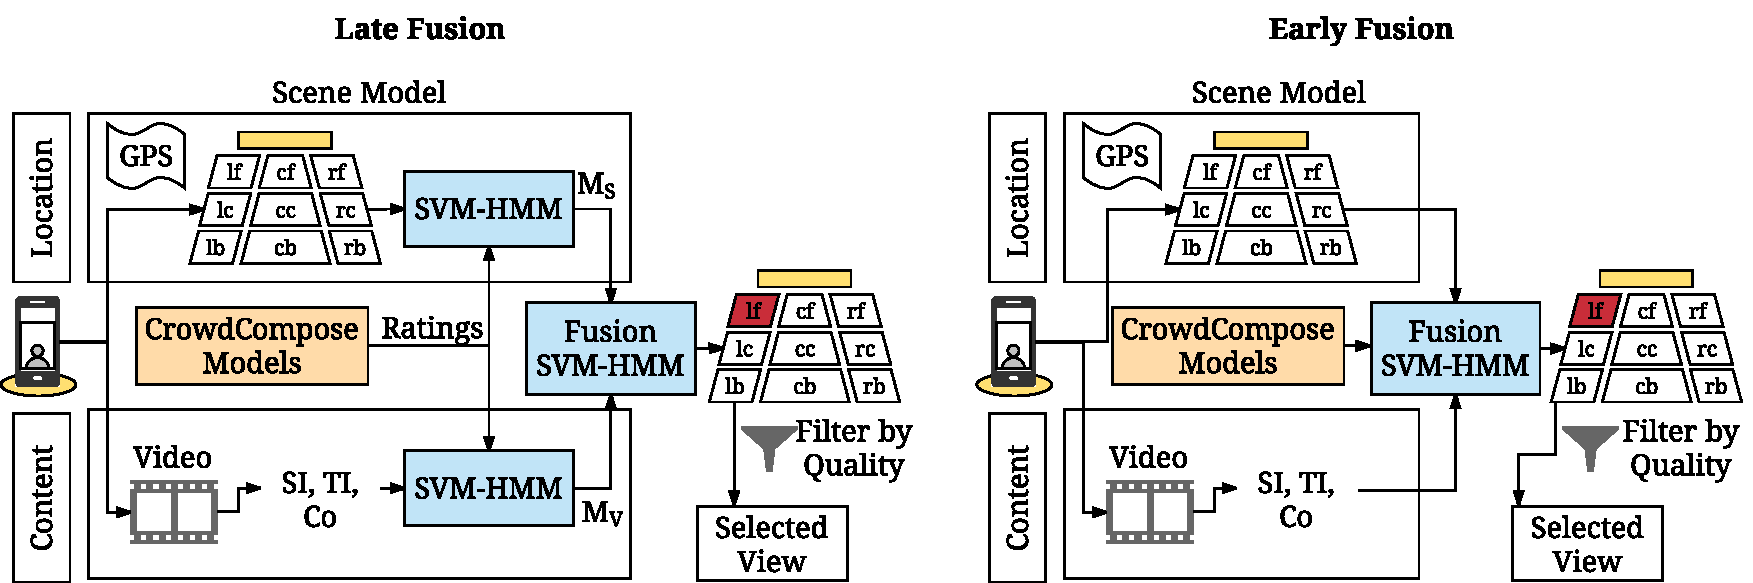
\includegraphics[width=\linewidth]{./gfx/600_Composition/svm_hmm_autocompose_fusion_step1}}\\
	\subfloat[]{
\includegraphics[width=\linewidth]{./gfx/600_Composition/svm_hmm_autocompose_fusion_step2}}	
	\caption[Concept of AutoCompose]{Concept of AutoCompose for automatic video composition: (a) Overview on the process of early fusion-based view selection in comparison with the late fusion for determining the next view and (b) Process to determine the video shot duration.}
	\label{fig:630_viewSelection}
\end{figure}
\subsection{Early Fusion versus Late Fusion}
Figure~\ref{fig:630_viewSelection} depicts different approaches for learning and predicting video compositions.
The approaches are based on the concepts of early and late fusion of feature vectors~\cite{Snoek2005}.
A fusion decision has to be made if features stem from different modalities.
Early fusion combines the different features in a single feature vector representation and trains the \ac{SVM-HMM}.
This combination is achieved by concatenating the features~\cite{Snoek2004}.
For the recording position selection, this would mean that the genre, content characteristics, and recording location are depicted in a single model.
The trained \ac{SVM-HMM} can then be used for predicting the next compositions.

The late fusion separates the features into their modalities, e.g., the location independent of video characteristics, and trains different \ac{SVM-HMM}s. 
Thus, individual models first learn in an initial stage the semantics of the video composition, independent of each other.
Probabilities or tag sequences retrieved from the first-stage \ac{SVM-HMM} are then fused in a second stage \ac{SVM-HMM}.
The second stage gives the final result of the prediction.
Early fusion is also described as the fusion of  modalities in the feature space, whereas the late fusion is described as a fusion in the semantic space~\cite{Snoek2005}.

In the conducted evaluations, late fusion has shown a negligible improvement of the correct classification rate for the JIKU video dataset~\cite{Saini2013}.
The correct classification rate slightly decreased from 81.3\% in the early fusion to 80.9\% in the late fusion. 
At the same time, the learning and prediction time nearly doubled - making such an approach unfeasible for live video composition.
The evaluated version of AutoCompose relies on the early fusion approach.